\chapter{Dynamic structures for data of any type}
\begin{refsection}

\abstract{This unit provides abstract LIFOs and FIFOs that can be used with any data type. }

\begin{figure}
 \caption{\capstart Dynamical data structures: stack (\emph{green}), queue (\emph{pink}) and binary tree (\emph{yellow}). For details see text. }
 \label{fig:Dynam}
 \centering
 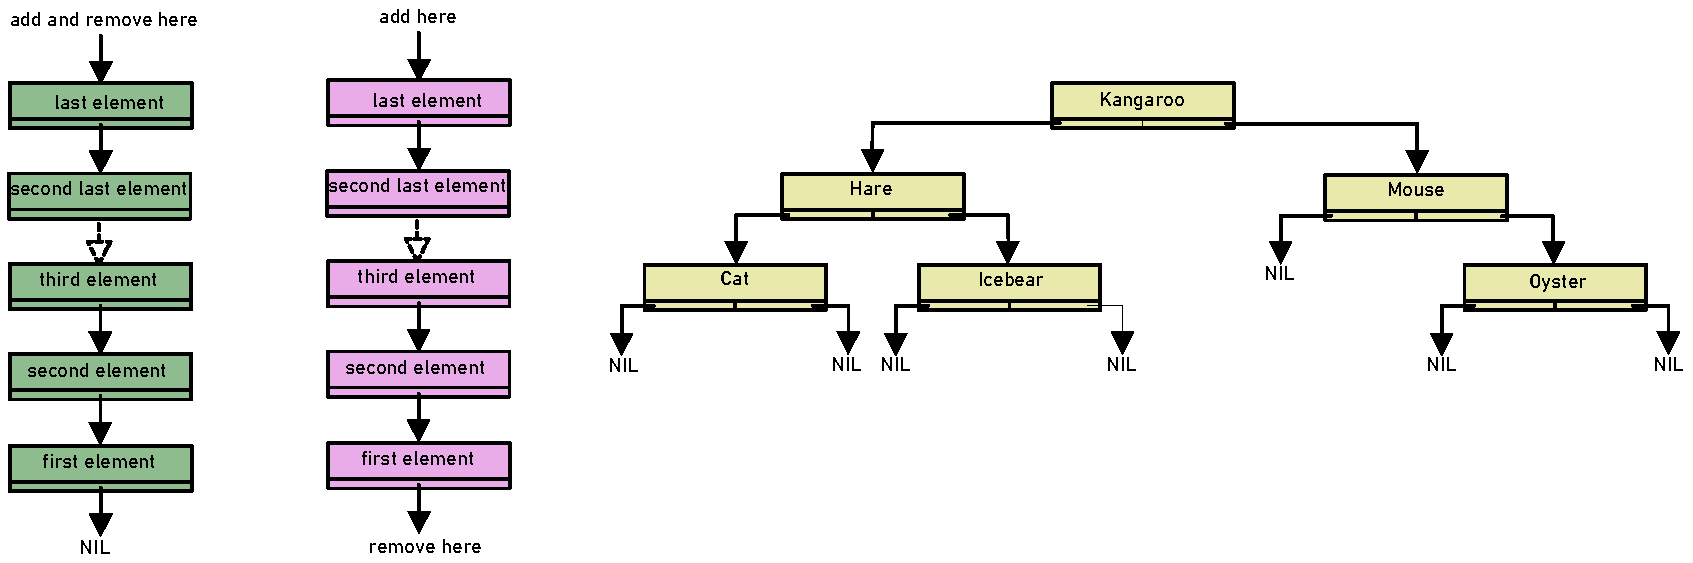
\includegraphics[width=\textwidth]{Graphics/Dynamical}
\end{figure}

This unit provides abstract data structures that can be used to store data of any type (\texttt{procedure Store(var I; S : word);}). The variable \texttt{I} is untyped (more correctly: can have any type). Untyped parameters of functions and procedures were not part of the original \texttt{Pascal}-definitions, they were introduced in \texttt{Turbo-Pascal 4}. From the point of view of this unit, \texttt{I} is simply an \texttt{array [S] of byte}, where \skalar{S} is the number of bytes required (obtained with \texttt{SizeOf()}). This unit was modified from \parencite{Sch-89}. An implementation of abstract binary trees has been published in \parencite{Arb-12}, but isn't needed for this project.

\section{The interface}

\begin{lstlisting}[caption=Interface of unit Dynam]
  UNIT Dynam;

  INTERFACE

  USES MathFunc; // here used only for error handling

  CONST DynamError : BOOLEAN = FALSE;
        MaxElem    = 2000;

  TYPE
    Space = ARRAY[0..MaxElem] OF BYTE;

  { ***************************** LiFo ***************************** }

    LList = ^LListNode;

    LListNode = RECORD
      Size: WORD;
      Info: ^Space;
      Next: LList;
    END;

    LIFO = LList;

  PROCEDURE InitLIFO(VAR L: Lifo);
  {einen leeren Stapel initialisieren}

  FUNCTION EmptyLIFO(L: LIFO): BOOLEAN;
  {pr��fen, ob der Stapel L leer ist}

  PROCEDURE PUSH(VAR L: LIFO; VAR I; S: WORD);
  {einen Wert auf den Stapel legen}

  PROCEDURE POP(VAR L: Lifo; VAR I; S: WORD);
  {einen Wert aus dem Stapel nehmen}

  { ***************************** FiFo ***************************** }

  TYPE
    FList = ^FListNode;

    FListNode = RECORD
      Size: WORD;
      Info: ^Space;
      Next: FList;
    END;

    FIFO = RECORD
      First, last: FList;
    END;

  PROCEDURE InitFIFO(VAR F: FIFO);
  {legt eine leere Schlange an}

  FUNCTION EmptyFIFO(F: FIFO): BOOLEAN;
  {true, wenn die Schlange leer ist}

  PROCEDURE Put(VAR F: FIFO; VAR I; S: WORD);
  {einen Wert I mit Gr��e S in die Schlange schieben}

  PROCEDURE Get(VAR F: FIFO; VAR I; S: WORD);
  {einen Wert I der Gr��e S aus der Schlange holen}

  {****************************************************************************}

  IMPLEMENTATION
  
  VAR ch : char; // for error handling
\end{lstlisting}

\section{The LIFO (stack)}

A LIFO resembles a stack of dinner plates, new plates are added (\texttt{Push}) to the top and also required plates are removed (\texttt{Pop}) from the top (see fig. \ref{fig:Dynam}, \emph{left}). The only two other operations allowed are the creation of a new stack (\texttt{InitLIFO}), and freeing the space of an empty stack (\texttt{EmptyLIFO}).

The items in the stack are linked by pointers. The pointer to the stack points to the top element, which contains a pointer to the next element and so on. When an element is removed from the stack, the pointer to the next element becomes the pointer to the stack; if, on the other hand, an element is added the pointer to the former top becomes its pointer to the next element and the new pointer to the stack points to the new element. At the end of the stack the pointer from the last element (the one added first) is \texttt{NIL}. When the last element has been reached, the pointer to the stack therefore becomes \texttt{NIL}.

\begin{lstlisting}[caption=LIFO]
  PROCEDURE InitLIFO(VAR L: LIFO);


  BEGIN
    L := NIL;
  END; (* InitLIFO *)


  FUNCTION EmptyLIFO(L: LIFO): BOOLEAN;

  BEGIN
    Result := L = NIL;
  END; (* EmptyLIFO *)


  PROCEDURE PUSH(VAR L: LIFO; VAR I; S: WORD);

  VAR
    p: LList;

  BEGIN
    NEW(p);
    WITH p^ DO
      BEGIN
        Size := S;
        Next := L;
        GetMem(Info, Size);
        Move(I, Info^, Size);
      END; (* WITH *)
    L := p;
  END; (* Push *)


  PROCEDURE POP(VAR L: LIFO; VAR I; S: WORD);

  VAR
    p: LList;

  BEGIN
    p := L;
    WITH p^ DO
      BEGIN
        IF Size <> S
          THEN
            BEGIN
              Writeln('TYPE-MISMATCH-ERROR');
              HALT;
            END;
        Move(Info^, I, Size);
        FreeMem(Info, Size);
        L := Next;
      END; (* WITH *)
    DISPOSE(p);
  END; (* Pop *)
\end{lstlisting}

\section{The FIFO (list, buffer, queue)}

If the new mail reaching an office would be added to a \texttt{LIFO}, the mail at the bottom may never be answered.  Therefore, in a queue, the elements are added from one end (\texttt{Put}) and removed from the other (\texttt{Get}). Such a list has two pointers, one for the beginning and the other for the end. The pointer from the element added first is \texttt{NIL} (see fig. \ref{fig:Dynam}, \emph{middle}).

\begin{lstlisting}[caption=FIFO]
  PROCEDURE InitFiFo(VAR F: FiFo);

  BEGIN
    WITH F DO
      BEGIN
        First := NIL;
        last := NIL;
      END;
  END;


  FUNCTION EmptyFiFo(F: FiFo): BOOLEAN;

  BEGIN
    Result := F.First = NIL;
  END;


  PROCEDURE Put(VAR F: FiFo; VAR i; s: WORD);

  VAR p: FList;

  BEGIN
    NEW(p);
    WITH p^ DO
      BEGIN
        Size := S;
        Next := NIL;
        GetMem(Info, Size);
        Move(I, Info^, Size);
      END;
    IF EmptyFiFo(F)
      THEN
        BEGIN
          F.First := p;
          F.last := p;
        END
      ELSE
        BEGIN
          F.last^.Next := p;
          F.last := p;
        END;
  END;


  PROCEDURE Get(VAR F: FiFo; VAR i; s: WORD);

  VAR
    p: FList;

  BEGIN
    p := F.First;
    WITH p^ DO
      BEGIN
        IF Size <> s
          THEN
            BEGIN
              Writeln('Type-Mismatch-Error');
              HALT;
            END;
        Move(Info^, I, Size);
        FreeMem(Info, Size);
        F.First := Next;
      END;
    DISPOSE(p);
  END;
\end{lstlisting}




\section{Test-program}

The following program tests the data structures provided by \texttt{Dynam} and demonstrates how they can be used.

\begin{lstlisting}[caption=Test program]
PROGRAM TestDynam;

USES dynam, mathfunc, crt;


PROCEDURE LifoFifoTesten;

VAR s          : STRING[20];
    LifoListe  : Lifo;
    FifoListe  : Fifo;
    i          : WORD;

BEGIN
  ClrScr;
  Writeln('Demoprogramm f�r die Arbeit mit Fifo und Lifo-Strukturen');
  Writeln;
  InitLifo(LifoListe);
  InitFifo(FifoListe);
  Writeln('Bitte geben Sie jetzt 10 kurze Strings ein (z.B. Namen)');
  Writeln;
  Writeln('EINGABE', 'AUSGABE von LIFO': 30, 'AUSGABE von FIFO': 30);
  Writeln;
  FOR i := 1 TO 10 DO
    BEGIN
      ReadLn(s);
      PUSH(LifoListe, s, SizeOf(s));
      Put(FifoListe, s, SizeOf(s))
    END;
  GotoXY(1, 7);
  WHILE NOT EmptyLifo(LifoListe) DO
    BEGIN
      GotoXY(30, WhereY);
      POP(LifoListe, s, SizeOf(s));
      Writeln(s)
    END;
  GotoXY(1, 7);
  WHILE NOT EmptyFifo(FifoListe) DO
    BEGIN
      GotoXY(60, WhereY);
      Get(FifoListe, s, SizeOf(s));
      Writeln(s)
    END;
  Writeln;
  Writeln('weiter mit RETURN:');
  ReadLn;
END; {LifoFifoTesten}

TYPE KeyType = WORD;

BEGIN  // Test program
  LifoFifoTesten;
END.
\end{lstlisting}

\printbibliography[heading=subbibliography]
\end{refsection}









































































































